\section{Related work}
\subsection{Extracting data from software repositories}

Mining repositories to extract knowledge from them has been an object of study for several years.

In \cite{Ying_2004} it is proposed an approach that, when developers are editing a file, recommends other files that may also need edits. This is done by analyzing which files have frequently changed together in the past (using a version control system), and applying a frequent pattern mining algorithm to them. For a better analysis, they consider not only files that were committed together, but also files that were committed by the same author in a short period of time, as they most likely refer to the same task. Finally, they also filter commits with too many files changed, as these commits usually don't refer to a single task and so aren't relevant for recommendations.

A frequent pattern mining algorithm is also used in \cite{Kagdi_2007}. The knowledge of files frequently changed together (called "change sets") is used to uncover "traceability between source code and other artifacts", like documentation. They also use heuristics like changes in a small period of time ("\textbf{time-interval}"), changes by the same author ("\textbf{committer}"), and a mix of both ("\textbf{time-interval + committer}") to group change sets that probably refer to the same task/change. By evaluating the approach on several versions of \textit{KDE} (K Desktop Environment), the authors find that this approach is able to find links between different types of artifacts like "source code files, change logs, user documentation, and build files" with high accuracy.

In \cite{Alali_2008}, an analysis of different metrics of commits like number of changed files, number of changed lines and hunks (which are groups of lines that changed, together with contextual lines that did not) is done to categorize a commit from "extra small to extra large". The categorization of a single commit is always done relative to predefined criteria, obtained from all commits of the same repository. This predefined criteria is obtained (for each metric) by calculating the statistical 5-point summary (Minimum, Q1, Median, Q3, Maximum). Plotting these values into a Boxplot allows for a division into 5 regions, as seen in figure \ref{fig:boxplot-commit-size}. A single commit is then classified according to where the metrics fall in this Boxplot.

\begin{figure}[h]
    \centering
    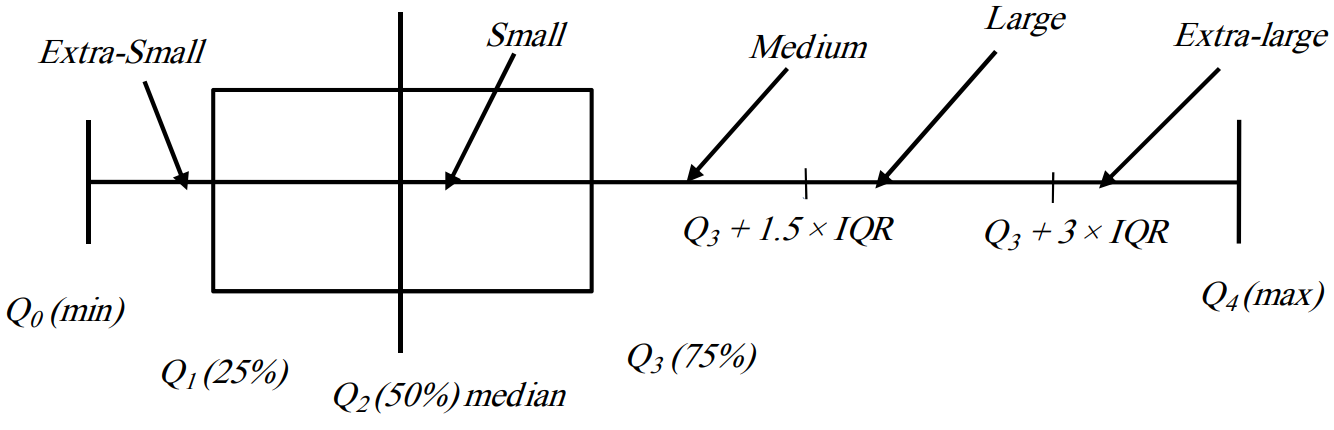
\includegraphics[scale=0.2]{imgs/boxplot-commit-size.png}
    \caption{Boxplot of the regions for classification of commit size. From \cite{Alali_2008}}
    \label{fig:boxplot-commit-size}
\end{figure}

Applying this to the commits of nine open source repositories (of various sizes and languages), and using messages in commits' log files to determine the activity performed, let the authors conclude that there is some evidence the category of a commit can indicate the activity being performed. For example, extra-small commits typically have the set of words \{add, bug\} in their messages.

The problem of assigning the best code reviewer(s) to a given pull request affects many players in the industry, with \cite{Yu_2016} mentioning that "the management of pull requests is identified as the most important project activity on GitHub". Different authors try to solve this problem with past software history change analysis. A tool called "Review Bot" was developed in \cite{Balachandran_2013} mainly to aid code reviewers in the process of reviewing pull requests, by using static analysis techniques to check for code style violations and bad patterns. The tool also recommends code reviewers based on \textit{line change history}, and it does so with an accuracy of 60\% to 90\%. Another approach to recommend reviewers, but based on file paths, is described in \cite{Thongtanunam_2015}. The tool they propose is applied to a new review, and the recommendations are based on who reviewed similar file paths in the past as the ones changed in that review. Finding similar file paths is done by string comparison techniques, like \textbf{Longest Common Prefix} (files under the same directory are considered similar), \textbf{Longest Common Suffix} (files with the same name are considered similar), \textbf{Longest Common Substring} and \textbf{Longest Common Subsequence} (files under a similar directory structure are similar). This approach was evaluated on a total of 42,045 reviews across 5 different open source projects (Android Open Source Project (AOSP), OpenStack, Qt and LibreOffice), and it "correctly
recommended 79\% of reviews with a top 10 recommendation" - 3 times better than ReviewBot.


Both of these papers address the issue by ultimately assuming that developers who changed a file most often have the most familiarity and expertise in that file. However, \cite{Schuler_2008} assume that developers who use a \textit{functionality} most often, by calling a method, are the most familiar with it. They introduce the notion of \textit{usage based expertise}, which, together with \textit{implementation based expertise} (those who modified methods are most familiar with them), is used to create \textbf{expertise profiles}. To build this profile for a developer, they looked at and counted all the methods that the developer changed (or added) and used in past commits. Then, it's easy to find developers who have experience with using a given module - it's a matter of considering a set with all methods of that module, and counting intersections with profiles. One application mentioned in the paper is in the calculation of neighborhoods of developers - sets of developers with the most similar expertise. This could help with the creation of teams (with members from different projects) to discuss usage of an API, or with scheduling meetings with developers working on "related parts of the code", or even "to choose developers for training of their skills", by identifying who would need training in a given technology the most.


There are also other interesting conclusions and associations that can be extracted with the data of different repositories. Not much is known regarding what happens to the code quality of programmers very familiar with a language when they switch to another they don't use that often. This is explored in \cite{Horschig_2018}, where the authors searched in a GitHub dataset for Java and C++ programmers that occasionally program in Python, and studied their Python code quality with a lint tool. They found, for example, that C++ programmers usually write more complex methods in Python than a control group, and they tend to use loop variables outside of a loop more often. Java programmers tend to redefine outer names more times than Python programmers, and both C++ and Java programmers write longer lines.
% Este paper do Horschig usou o GHTorrent. Será preferível mencionar isso, e meter o GHTorrent num parágrafo anterior?

Stack Overflow (SO) is an ever-present website in developers' lives, with many snippets available for solving both common and unique problems. In \cite{Yang_2017}, the presence of SO snippets in real projects, and what adaptations (if any) these snippets had is studied. They analyzed 909k non-fork Python projects, and found that the percentage of snippets found both in SO and GitHub (GH) is low - under 2\% of analyzed snippets, which results in just thousands of snippets. Nevertheless, there is some evidence of code flow from SO to GH.


Measuring developer contribution in an agile and distributed development context is not a trivial task. According to \cite{Gousios_2008}, "an important portion of development time is spent on communication and manipulation of development support tools". Therefore, a new model for contribution measurement was developed and explained, which mixes repository data with traditional contribution metrics (lines of code) to get a more accurate contribution measure. The model is based on a function that applies weights to different actions on a repository. Committing translation files, including a bug report number on a commit message, or committing documentation files are examples of code-related actions. However, there are also non code-related actions, like creating or updating a new Wiki page, participating in IRC (keep in mind the paper was published in 2008), replying to a mailing list thread, or closing a bug. All of these are associated with positive weights, but there are some actions with negative weights - closing a bug that is then reopened, committing without messages, making large commits (with more than \textit{X} files), or making commits that generate bugs. To compute the weights, the authors first compute clusters of similar projects, since certain types of projects are expected to have more actions of certain types than others. Then, all of the considered events are counted across all projects of each cluster, and the weight $w_i$ for each action is "the percentage of contribution of each action category to the total number of actions". Manual weights are applied to the sum of all $w_i \times action_i$ for actions of a given type. These manual weights are chosen according to the needs of each project. This offers a contribution factor that is applied to developers and is summed to their total Lines of Code (LOC), resulting in a modern contribution metric.

% Não estou muito inspirado neste parágrafo
%According to \cite{Gong_2021}, code authorship attribution is an important research topic, with applications ranging from bug report assignments and software forensics to plagiarism detection. In the same paper, the revision histories and past contributions of developers are leveraged to try to find hidden code authors. This was done with an empirical evaluation, by developing a tool called CodA which evaluated in total 12092 files written by 506 programmers, in six Java projects. In total, they reported 7 findings. For example, if all lines written by author $A$ in source file $S$ are replaced in later commits, then it's not legitimate to say that $A$ is still an author of $S$.


\cite{Gousios_2013} released the "GHTorrent Project", also available online\footnote{\url{https://ghtorrent.org/}}. Through a decentralized way, all data from GitHub events (like new commits, new authors, new issues - everything that may happen in a repository) is stored in a standardized form in a database.
This way, researchers can scale their findings to many repositories, as well as combine data from different repositories more easily, as it's a matter of performing queries on a database rather than using an API. The paper also presents several research opportunities, like ...

\cite{Seker_2020} investigated 172 studies that used this database, and categorized them into several software engineering domains and the challenges they addressed in those domains. The domains considered and some of their challenges are found below:

\begin{itemize}
    \item User
        \begin{itemize}
            \item \textit{Activity}. Covers developer's contributions, like coding history, comments, and stars in repositories.
            \item \textit{Revision - Assignment}. Everything that deals with pull request (PR) reviewer or bug assignment.
        \end{itemize}
    \item Development
        \begin{itemize}
            \item \textit{Pull Request and Quality}. Covers problems with pull request prioritization, and acceptance/rejection and reasons for it.
        \end{itemize}
    \item Project
        \begin{itemize}
            \item \textit{Issue/bug}. Includes topics of open and closed issues in a project and bug occurrences, as well as the classification of issue-bug-feature.
            \item \textit{Dependency}. Contains examinations of dependencies on GitHub projects on programming languages, codes, forking cases...
        \end{itemize}
    \item Dataset
        \begin{itemize}
            \item \textit{Helper}. Studies that used only a few features of GHTorrent to solve dissimilar problems.
            \item \textit{Subset}. Studies created by filtering the dataset according to certain features of developers or projects.
        \end{itemize}
\end{itemize}

The study also presented several pros and cons of GHTorrent, as well as challenges found using it. For example, GHTorrent is very flexible as it presents data in different formats (JSON in a MongoDB database and relational tables in MySQL database). However, it contains some duplicated data, it is missing some fields that could link data (like the \textit{repo id} in commits), and it does not have data on who edited what file.

\subsection{Summary}
Table \ref{tab:software-history-usage} summarizes what particular part of the software repositories the previously described studies use.

%Se calhar remover a coluna da granularidade?

\begin{table}[h!]
    \centering
    \caption{Summary of the usage of software history}
    \tiny
    \begin{tabular}{|P|L|L|L|L|}
        \hline
         Paper & Information Used  & Area & Strategy \\
         \hline
         \cite{Ying_2004} & Files frequently changed together, Committer, Time of commit & File editing recommendation & Identify and filter atomic change sets, apply frequent pattern mining, query when editing a file \\
         \hline
         \cite{Kagdi_2007} & Files frequently changed together, Committer, Time of commit & Uncover traceability links & Identify and group change sets, apply frequent pattern mining, analyze patterns \\
         \hline
         \cite{Alali_2008} & Files commited, lines changed, hunks & Categorization of a normal commit in a repository & Statistical 5-point summary of all commits, and evaluation of a single commit with this summary \\
         \hline
         \cite{Balachandran_2013} & Past pull requests (PR) changes and reviewers & Pull request reviewer assignment & Check reviewers of past PR containing each line in a new PR diff  \\
         \hline
         \cite{Thongtanunam_2015} & Past PR files' paths and reviewers & Pull request reviewer assignment & Compute a score for string similarity of files' paths in previous reviews and the new review, add that score to all reviewers in the previous reviews, display ranks\\
         \hline
         \cite{Schuler_2008} & Changed and inserted methods in commits & Pull request reviewer assignment & Group commits in a sliding time window approach, create two Abstract Syntax Trees (before and after the commit), store changed and implemented methods and their authors \\
         \hline
         \cite{Horschig_2018} & Files in a snapshot & Off-Language Code Quality & Java and C++ programmers that use Python, as well as Python programmers, were selected. The state of their projects at the time of writing was analyzed with \textit{PyLint}, and statistical conclusions drawn. \\
         \hline
         \cite{Yang_2017} & Files in a snapshot & Code flow from StackOverflow to GitHub & Blocks are extracted from source code (with an AST) and SO posts, and then tokenized. Blocks and tokens are hashed and compared, and a tool is used to detect missed similarities in blocks\\
         \hline
         \cite{Gousios_2008} & Lines and files committed, authors, Mailing lists/Forum, Bug Database, Wiki, IRC & Developer contribution & The events to be considered are counted, and weights are attributed to the values to create a Contribution Factor. \\
         \hline
    \end{tabular}
    \label{tab:software-history-usage}
\end{table}


\subsection{Related work in migration}

A comprehensive Systematic Literature Review (SLR) of service identification approaches (SIAs) for legacy software systems modernization, covering 41 SIAs, was done in \cite{Abdellatif_2021}. As this study was published in 2021, it offers an updated view of the state of the art in regards to the techniques being explored for the identification of services in legacy software systems, and the modernization of these systems to a Service Oriented Approach (SOA). Three different generic strategies for this migration are presented. The first one is a \textit{top-down}, forward-engineering approach: the domain artifacts are decomposed at a high-level, the services of the final SOA are modeled and then implemented, and the process to orchestrate them is then implemented at the end. The second one is a \textit{bottom-up} approach: the dependencies of the legacy system are extracted, the existing applications are mined to find the reusable functionality that could be a service, the functionalities are then packaged as services (without dependencies) and then existing applications are rewritten to use the new services. The third and final approach is a \textit{hybrid} one: the functions of the application are grouped into blocks, the blocks are mapped to available services while removing dependencies, and the process to orchestrate the services is implemented. Most of the reviewed literature in this SLR focuses on \textit{bottom-up} and \textit{hybrid} approaches - this is due to the fact that, most often, companies only have the source code of the legacy system as the most up-to-date information of said system.

The inputs to SIAs can be classified into three categories: executable models of the systems (source code, database schemas and test cases), non-executable models of the systems (runtime artifacts extracted as the system is running like Log Traces and User Application Interaction, and non-executable artifacts describing the architecture, like Business Process Models, Activity Diagrams and State Machine Diagrams) and domain artifacts (software documentation, human expertise, and ontologies). Most of the inputs are the source code, for reasons mentioned before.

As the present work aims to focus more on the usage of commits as a means to identify services, we will explore more deeply what has been done in the literature in this regard. In \cite{Mazlami_2017}, a model for microservice extraction using the software change history of a monolith is presented. First, an existing codebase making use of a version control system is analyzed to extract sets that characterize the monolith: the set of class files $C_M$, the set of the change history $H_M$, and the set of developers that committed code $D_M$. $H_M$ is composed of several change events $h_i$. Each one contains the set of classes from $C_M$ that were added or modified, $E_i$, as well as the timestamp $t_i$ in which the event happened, and the developer $d_i$ that committed the change. Once all of these are defined, a \textit{coupling strategy} is used to create an "undirected, edge-weighted graph", where the vertices correspond to a class from $C_M$. Edges indicate coupling between classes, and have a weight that defines how strong that coupling is. Once the graph is obtained, a clustering algorithm is applied to get a recommendation for microservices. The authors define three coupling strategies. (1) \textit{Logical Coupling} is based on the assumption that if development follows the Single Responsibility Principle, then a software component should only have one reason to change: as such, software elements that change together do so for the same reason. This leads to the conclusion that class files that change together should belong to the same microservice. To build the graph using this strategy, the number of times each two distinct classes were changed in the same change event is counted. The obtained value is used as the weights for the edges connecting those two classes. (2) \textit{Semantic Coupling} is based on a rationale that states that each microservice should match a context from the problem domain. To achieve this, classes that contain code about the same domain model entities should belong to the same microservice. To find those classes, each pair of distinct classes is analyzed. The files containing the classes are tokenized, and unwanted tokens like programming language symbols or identifiers are removed. A term list is created by combining the words from both class files, and is used for the computation of the two term-frequency inverse-document-frequency (tf-idf) vectors, $X$ and $V$. The weight of the edge connecting the two classes is given by the cosine of the two vectors $X$ and $V$. (3) \textit{Contributor coupling} follows from the microservice principle of cross-functional teams, centered around domain and business capabilities. The goal is to reduce communication overheard with external teams as much as possible, and to maximize internal cohesion and communication between developer teams of the same service. Therefore, it makes sense to separate microservices according to who works on them. To implement this strategy, all change events that modified a given class are first found. Then, the set of all authors that contributed to those events are computed. The weight of an edge is given by the cardinality of the intersection of the sets of developers that worked on the vertices of that edge. The performance of the different approaches, as well as combinations of them, was evaluated on 21 different projects. The projects were web-applications written in Java, Python, and Ruby, and use an ORM-technology for data management. Generally, the semantic coupling strategy took the longest time to run, and as expected, directly depended on the LOC. Logical coupling's execution time rised with the number of commits, and contributor coupling was mostly impacted by the history size (with some outliers where the number of classes has a greater impact). To evaluate the quality of the proposed separation, the authors considered two metrics. \textit{Team size reduction ratio} (\textit{tsr}) refers to what happens with the team size after the migration - values lower than 1 indicate a reduction in team size. This is a desired outcome, as it implies reduced communication overhead and as such more time can be spent in the actual domain problem. The ratio is computed by dividing the average team size across all microservices candidates, and the team size of the original monolith. % Como é que se calcula o team size?
All of the strategies (and combinations) had a median value below 0.5, so all approaches performed well according to this metric. It's worth noting that for the contributor coupling strategy, certain events may lead to a \textit{tsr} of 1. For example, if there's a certain class file that all contributors in the history of the project have changed, then by definition, that file will be coupled to every other class file in the monolith. This leads to the clustering algorithm returning a single microservice candidate, which has the same teamsize of the original monolith since it contains all contributors of the monolith. The second metric, \textit{Average Domain Redundancy}, concerns itself with whether there is domain-specific duplication or redundancy between the services. The value is normalized between 0 and 1, and a lower value is better: it means that the services are more isolated and just do a specific task, as they ideally should. The contributor coupling strategy was the only one above 0.25, while the remaining ones were all below 0.25. When using this strategy (either alone or in combination with others) the upper quartile tended to be very high. This happened because in open-source projects, developers' skill distribution is technology oriented, and not domain oriented - front-end developers contribute to the same files, independent of their domain content. Back-end and database developers do the same. Therefore, this leads to class files existing in the same microservice despite their low semantic and domain-specific cohesiveness.
Overall, the semantic coupling performed the best in this metric. This makes sense, as it's the only strategy that actually looks at the domain when building the graph. The results show that the strategies by themselves, and their combinations, perform very well by being able to reduce the microservice team size, and lowering the average domain redundancy.

In \cite{Santos_2021}, a mixed approach between static analysis and the software change history is proposed.